\chapter{Axioms and Derived Variables}\label{ch:axioms}
\chapterquote{The grand aim of all science [is] to cover the greatest number of empirical facts by logical deduction from the smallest possible number of hypotheses or axioms.}{Albert Einstein (1950)}

\renewcommand{\kiviatPredicates}{2}
\begin{figure}[t]
    \begin{center}
        \begin{tikzpicture}
    \tkzKiviatDiagram[
    radial style/.style ={-{Latex[length=3mm, width=2mm]}},
    scale=0.85,
    label space=1.5,
    radial = 1,
    gap = 1.5,
    step = 1,
    lattice = 2]{
    \hspace{2.5cm}\mbox{\parbox{4cm}{{\begin{center}\textbf{Goal}\\\textbf{Description} \end{center}}}},
    {\textbf{Number of Plans}},
    \hspace{-1.5cm}\mbox{\parbox{3cm}{{\begin{center}\textbf{State}\\\textbf{Description}\end{center}}}},
    \textbf{Cost Function}}

    \ifbool{kiviatRed}{
        \tkzKiviatLine[very thick,color=red!50,
            fill=red!30,
            opacity=.35,
            mark=ball,
            mark size=2.5pt,
            ball color=red](\kiviatGoal{},\kiviatTopk{},\kiviatPredicates{},\kiviatCost{})
    }

    \ifbool{kiviatBlue}{
        \tkzKiviatLine[very thick,color=blue!50,
            fill=blue!30,
            opacity=.35,
            mark=ball,
            mark size=2.5pt,
            ball color=blue](1,1,1,1)
    }

    \ifbool{kiviatFull}{
    \tkzKiviatLine[very thick,color=darkgreen!50,
        fill=green!30,
        opacity=.35,
        mark=ball,
        mark size=2.5pt,
        ball color=darkgreen](1,2,2,2)
    \tkzKiviatLine[very thick,color=blue!50,
        fill=blue!30,
        opacity=.35,
        mark=ball,
        mark size=2.5pt,
        ball color=blue](1,1,1,1)
    \tkzKiviatLine[very thick,color=red!50,
        %fill=red!30,
        %opacity=.35,
        mark=ball,
        mark size=2.5pt,
        ball color=red](\kiviatGoal{},\kiviatTopk{},\kiviatPredicates{},\kiviatCost{})
    \LegendBox[shift={(-0cm,-2.25cm)}]{current bounding box.south west}%
    {
    red!100/{Forward symbolic search (contribution of this thesis)},
    asparagus!100/{Bidirectional symbolic search (contribution of this thesis)},
    blue!100/{Bidirectional symbolic search (previous state of the art)}}
    }
    {}

    % goal specification
    \draw[] node[align=center,fill=none] at (1.5,-0.5) {\small Hard};
    \draw[] node[align=center,fill=none] at (3.25,-0.75) {\small Oversub-\\ \small scription};
    %\draw[] node[] at (1.75,-0.6) {\rotatebox{-45}{hard}};
    %\draw[] node[align=center] at (3.85,-1.25) {\rotatebox{-45}{oversubscription}};

    % number of plans
    \draw[] node[align=center,fill=none] at (0.7,1.5) {\small Top-$1$};
    \draw[] node[align=center,fill=none] at (0.7,3.0) {\small Top-$k$};

    % derived predicates
    \draw[] node[align=center,fill=none] at (-1.25,0.75) {\small State\\ \small Variables};
    \draw[] node[align=center,fill=none] at (-3.25,0.75) {\small $+$ \small Derived\\ \small Variables};

    % cost function
    \draw[] node[align=center,fill=none] at (-1,-1.5) {\small Constant};
    \draw[] node[align=center,fill=none] at (-1.6,-3.0) {\small State-Dependent\phantom{0}};
\end{tikzpicture}
    \end{center}
    \caption[Overview of extension for classical planning (axioms).]{Overview of extensions for classical planning, where the red color denotes the planning formalism supported by the proposed symbolic search approach.}\label{fig:dervided_predicates:kiviat}
\end{figure}
\renewcommand{\kiviatPredicates}{1}

\section*{Core Publication of this Chapter}
\renewcommand{\citebf}[1]{\textbf{#1}}
\begin{itemize}
    \item \fullcite{speck-et-al-icaps2019}
\end{itemize}
\renewcommand{\citebf}[1]{#1}

In classical planning, Boolean or finite domain variables are used to describe the states of the world, the preconditions and the effects of actions, and the goal description \autocite{fikes-nilsson-aij1971,backstrom-nebel-compint1995}.
For many real-world problems, however, complex action preconditions or goals are desirable or even necessary for a compact problem description \autocite{thiebaux-et-al-aij2005}.
Axioms allow to model such complex preconditions and goals compactly by introducing a set of derived variables whose values are not directly influenced by the actions but are derived from the values of other variables using a set of logical axioms.
%\textcite{thiebaux-et-al-aij2005} showed that axioms are an essential feature because it is impossible to compile them away, i.e., to express them in the original formalism, i.e., as classical planning task (Definition \ref{def:planning-task}), without a super-polynomial growth of the plan length or description size.

Although axioms are an essential feature \autocite{thiebaux-et-al-aij2005} of \pddl{} \autocite{mcdermott-et-al-tr1998,hoffmann-edelkamp-jair2005}, the common language for modeling planning tasks, modern planning techniques rarely support axioms, especially in cost-optimal planning.
Most admissible heuristics commonly used in \astar{} search, one of the most prominent approaches to cost-optimal planning, are not defined for their use with axioms.
The few heuristics that support axioms are based on naive relaxations that consider axioms as zero-cost actions, which may greatly reduce the informativeness of the heuristics.
One exception is the axiom-aware delete relaxation heuristic, obtained by applying a model for state constraints to planning with axioms \autocite{ivankovic-haslum-ijcai2015,haslum-et-al-jair2018}.
While these heuristics are often informative, they are also time-consuming to compute and therefore often do not pay off in terms of coverage or runtime. 
%Moreover, to the best of our knowledge, other planning techniques, such as planning as satisfiability \autocite{kautz-selman-ecai1992,rintanen-aij2012} and symbolic search \autocite{cimatti-et-al-ecp1997,torralba-et-al-aij2017} have not yet been extended to planning with axioms.

In this chapter, we define and motivate planning with axioms and summarize the known complexity and compilability results for this setting.
Then we describe three different sound and complete ways to extend symbolic search algorithms to support axioms natively introduced by \textcite{speck-et-al-icaps2019} (Figure \ref{fig:dervided_predicates:kiviat}).
%More precisely, three different ways of encoding axioms and derived variables with symbolic representations are analyzed.
The empirical study on different planning domains shows that the symbolic axiom encodings of \textcite{speck-et-al-icaps2019} yield an optimal planner that supports axioms and compares favorably with other state-of-the-art methods.

\section{Formalism}
Planning with axioms extends the formalism of classical planning (\Cref{def:planning-domain,def:planning-task}) with a set of derived variables and axioms as follows \autocite{thiebaux-et-al-aij2005,helmert-2008}.

\begin{definition}[Planning with Axioms]\label{def:planning_axioms}
    A \emph{planning task with axioms} is a tuple $\task = \langle \domain, \init, \goal, \limit \rangle$ with $\domain = \langle \vars, \operators, \constcostfun, \derivedvars, \axioms \rangle$ that extends an ordinary planning task and domain with a set of \emph{axioms} $\axioms$ that is used to evaluate a set of \emph{secondary} or \emph{derived} propositional {variables} $\derivedvars$. Partial variable assignments such as the preconditions $\pre_o$ of operators $o \in \operators$ and the goal condition are defined over primary and secondary variables $\vars \cup \derivedvars$.
    A variable assignment $s$ is called a \emph{state} if it is defined for all variables in $\vars$, and an \emph{extended state} if it is defined for all variables in $\vars \cup \derivedvars$.
    With $\states$ we refer to the set of all states and with $\extendedstates$ to the set of all extended states.
    $\axioms$ is a finite set of axioms over $\vars \cup \derivedvars$. An \emph{axiom} has the form $h \leftarrow b$ where the head $h$ is a variable in $\derivedvars$ and the \emph{body} $b$ is a finite conjunction of positive or negative literals over $\vars \cup \derivedvars$.

    The set of axioms is partitioning into a totally ordered set of axioms layers $\axioms_1 \prec \dots \prec \axioms_i \prec \dots \prec \axioms_k$ with $i=1,\dots,k$. The layer of an axiom is defined by the
    layer of its head, which is determined by a partition of the set of derived
    variables into subsets $\derivedvars_1 \prec \dots \prec \derivedvars_k$.
    We assume that this partition forms a \emph{stratification}, i.e., that for all $i=1, \dots, k$, and for each $d_i \in \derivedvars_i$, it holds that (1) if $d_j \in \derivedvars_j$ appears in the body of an axiom with head $d_i$, then $j \leq i$ and (2) if $d_j \in \derivedvars_j$ appears negated in the body of an axiom with head $d_i$, then $j < i$.
\end{definition}

The semantics of axioms is as follows: (1) to evaluate a derived variable, only axioms in the current or previous layers have to be considered, and (2) axioms have negation-as-fault semantics, i.e., if a fact cannot be derived as true, it is assumed to be false in subsequent layers \autocite{speck-et-al-icaps2019}.
%Therefore, axiom layers have to be fully evaluated before a variable from that layer can be used negatively in another axiom body, which necessitates moving to a strictly higher layer if $d_j$ is used negatively . 
Given a state $s \in \states$ (over $\vars$), the extended state $\axioms(s) \in \extendedstates$ (over $\vars \cup \derivedvars$) is uniquely defined by the standard stratified semantics \autocite{apt-et-al-1988,thiebaux-et-al-aij2005}.
%
In other words, axioms are evaluated in a layer-by-layer fashion using fixed point computations.
More precisely, given a state $s \in \states$, first all derived variables $d \in \derivedvars$ are set to their default value (false), i.e., $\lnot d$. 
Second, a fixed point computation is performed for each axiom layer in sequence to determine the final values of the derived variables \autocite{helmert-2008}.
The evaluated derived variables together with the state $s$ form the extended state $\axioms(s)$.

Intuitively, the axioms form a background theory that makes it possible to capture/derive some properties of states, i.e., secondary variables, from the primary state variables.
Consequently, an operator can only change the values of the primary variables ($\eff_o$ is a partial variable assignment over $\vars$), and based on the primary variables in the successor state, the values of the secondary variables can be derived using the axioms.
Moreover, an operator is applicable in a state $s \in \states$ if $\pre_o \subseteq \axioms(s)$ and a state $s \in \states$ is a goal state if $\goal \subseteq \axioms(s)$.
For a detailed description and discussion of the semantics of axioms, see \textcite{thiebaux-et-al-aij2005,helmert-2008,helmert-jair2006}.
% Algorithm \ref{alg:axiom-explicit-evaluation} describes the axiom
% evaluation algorithm for explicit states, following the exposition of \intextcite{helmert-jair2006}. Some axiom
% definitions also specify a default value for derived variables, which is assumed
% before any rules are applied. We assume that the default value of all derived variables is $\bot$ (false).

%\todo{Maybe add explicit algorithm?}

\Cref{ex:axioms} illustrates the semantics and usefulness of axioms in the context of classical planning.

\begin{example}\label{ex:axioms}
    Consider the $\textit{navigate}$ operators of \Cref{ex:rover}, which navigates the rover from one cell to another with a cost of 0. This verbose modeling of the rover navigation leads to a larger state space and longer plan than necessary. Reachability can be expressed as a recursive property with axioms and derived properties.
    %
    To model a $\textit{navigate}$ operator with axioms that moves the rover to a reachable location $loc$, we introduce a derived variable $\textit{reachable(loc)}$ as a precondition for the $\textit{navigate}$ operator. The values for the derived variables $\textit{reachable(loc)}$ are determined by a single layer of axioms $\axioms_1$.
    \begin{itemize}
        \item $\textit{reachable(loc)} \leftarrow \textit{rover-at}=loc$
        \item $\textit{reachable(to)} \leftarrow \textit{reachable(from)} \land \textit{free(to)} \land \textit{adjacent(from,to)}$
    \end{itemize}

    Intuitively, the first axiom means that the current location of the rover is reachable. The second axiom means that a free location adjacent to a reachable location is also reachable. By applying the axioms until a fixed point is reached, the current state $s$ is expanded to $\axioms(s)$, which then contains the information about the actual reachable locations ($reachable(loc)$) based on the current state $s$, which contains the rover location and all relevant information about the map.
    This encoding provides a natural and concise modeling of the transitive closure property of reachability. Moreover, it provides not only a smaller state space, but also a shorter plan $\pi^\rover{} = \langle$\navigate{7}{1}, \startDrone{7}{1}, \fly{7}{1}{6}{1}, \takeImg{6}{1}, \fly{6}{1}{10}{1}, \takeImg{10}{1}, \fly{10}{1}{7}{1}, \landDrone{7}{1}, \navigate{0}{5}$\rangle$, which avoids the irrelevant choice of the exact path the rover must take.\footnote{If the navigation operators of the rover would have non-zero costs, such a modeling would require state-dependent action costs, which we discuss in more detail in \Cref{ch:sdac}.}
\end{example}

In \Cref{ex:axioms}, the reachable cells for the rover are always the same, but this is not necessarily true in general. For example, it could be possible that actions by the rover make some cells impassable.  A similar scenario where reachability can change from state to state is Sokoban, where the locations of the boxes affect the reachability of the cells \autocite{ivankovic-haslum-ijcai2015,miura-fukunaga-aaai2017}.

\section{Complexity and Compilability}

\textcite{helmert-2008} showed that planning with axioms (\Cref{def:planning_axioms}) is \PSPACE-complete, since it generalizes classical planning (hardness) and a non-deterministic Turing machine can solve the bounded plan existence problem for planning with axioms with polynomial space (completeness).

\begin{theorem}[\cite{helmert-2008}]
    Bounded plan existence of planning with axioms is \PSPACE-complete. \qed
\end{theorem}

\textcite{thiebaux-et-al-aij2005} show that axioms are an essential feature of the planning language \pddl{} \autocite{mcdermott-et-al-tr1998,hoffmann-edelkamp-jair2005}, proving that it is in general not possible to compile away axioms without a super-polynomial growth of the plan length or description size.\footnote{Note that \textcite{thiebaux-et-al-aij2005} also show that the 1-step planning with axioms problem is \EXPTIME{}-complete, which results from the fact that they consider planning tasks described in \pddl{}, while we consider planning tasks and, in particular, axioms in a grounded and normalized form.}
Furthermore, \textcite{thiebaux-et-al-aij2005} argue that axioms are necessary to model real-world problems in a compact and elegant way, as they allow to
model complex action preconditions (e.g. transitive closure property) or goals.
From these two observations, we can conclude that it is desirable and necessary to have search algorithms that can handle axioms directly with native support to solve some real-world problems.

\section{Symbolic Search}

\textcite{speck-et-al-icaps2019} introduce three different variants to support and represent axioms in symbolic search. All three encodings are sound and complete, allowing for optimal and complete symbolic search. We briefly describe the idea of the three symbolic variants and present an empirical evaluation comparing the symbolic approaches \autocite{speck-et-al-icaps2019} with explicit heuristic search approaches for planning with axioms \autocite{ivankovic-haslum-ijcai2015}. 
For a more detailed explanation of the symbolic encodings, we refer to \textcite{speck-et-al-icaps2019}.

\begin{figure}
    \centering
    \begin{tikzpicture}[>=latex]

    \node[] at (1,0) (dots) {\dots};
    \node[draw] at (3,0) (states) {$\charf_{S}$};
    \node[draw, diamond, aspect=1,align=center] at (7.0,0) (fixpoint) {fixed\\point?
    };
    \node[draw,align=center] at (10.0,0) (fullstates) {$\charf_{\{\axioms{}(s) ~\mid~ s \in S\}}$};

    \draw[->, thick] (dots) -- (states) node[pos=0.1,above,align=center] {apply\\operations};
    \draw[->, thick] (states) -- (fixpoint) node[midway,above,align=center] {apply\\axioms $\operators_{\axioms_i}$};
    \draw[->, thick] (fixpoint) -- (fullstates)  node[midway,above,align=center,xshift=-2pt] {yes};
    \draw[->,thick] (fixpoint.north) |- (6, 1.3) -| (states);
    \node[] at (5.0, 1.5) {no};

    \draw [decorate,decoration={brace,amplitude=10pt},xshift=-4pt,yshift=0pt,rotate=90]
    (-1.25,-7.5) -- (-1.25,-2.75) node [black,midway,below,yshift=-10pt,align=center]
    {\footnotesize for each axiom layer \\ $\axioms_{1}, \dots, \axioms_{k}$};
    \draw[->,dotted,thick] (fullstates) -- (12.0,0);
\end{tikzpicture}

    \caption[\operators{}-based encoding of axioms.]{Visualization of symbolic \emph{forward} search with the
        \operators{}-based encoding of axioms \autocite{speck-et-al-icaps2019}.\label{fig:axiom_option1}}
\end{figure}

% \begin{figure}
%     \begin{center}
%         \subfloat[$\operators$-based encoding of axioms.\label{fig:axiom_option1}]{
%             \begin{tikzpicture}[>=latex]

    \node[] at (1,0) (dots) {\dots};
    \node[draw] at (3,0) (states) {$\charf_{S}$};
    \node[draw, diamond, aspect=1,align=center] at (7.0,0) (fixpoint) {fixed\\point?
    };
    \node[draw,align=center] at (10.0,0) (fullstates) {$\charf_{\{\axioms{}(s) ~\mid~ s \in S\}}$};

    \draw[->, thick] (dots) -- (states) node[pos=0.1,above,align=center] {apply\\operations};
    \draw[->, thick] (states) -- (fixpoint) node[midway,above,align=center] {apply\\axioms $\operators_{\axioms_i}$};
    \draw[->, thick] (fixpoint) -- (fullstates)  node[midway,above,align=center,xshift=-2pt] {yes};
    \draw[->,thick] (fixpoint.north) |- (6, 1.3) -| (states);
    \node[] at (5.0, 1.5) {no};

    \draw [decorate,decoration={brace,amplitude=10pt},xshift=-4pt,yshift=0pt,rotate=90]
    (-1.25,-7.5) -- (-1.25,-2.75) node [black,midway,below,yshift=-10pt,align=center]
    {\footnotesize for each axiom layer \\ $\axioms_{1}, \dots, \axioms_{k}$};
    \draw[->,dotted,thick] (fullstates) -- (12.0,0);
\end{tikzpicture}

%         }\\\bigskip
%         \subfloat[$\vars$-based encoding of axioms.\label{fig:axiom_option2}]{
%             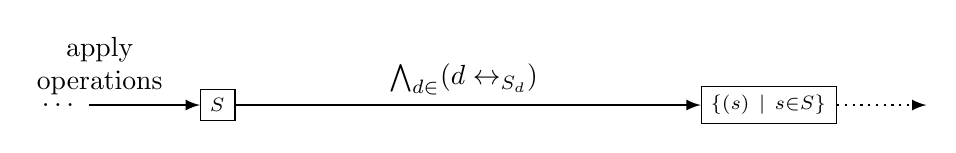
\begin{tikzpicture}[>=latex]
    %\node[draw,align=center] at (3.25, 1.75) {For all $d \in \derivedvars:$\\create BDD $S_d[\vars]$};
    \node[] at (1,0) (dots) {\dots};
    \node[draw] at (3,0) (states) {$\charf_{S}$};
    \node[draw] at (10.0,0) (fullstates) {$\charf_{\{\axioms{}(s) ~\mid~ s \in S\}}$};

    \draw[->, thick] (dots) -- (states) node[pos=0.1,above,align=center] {apply\\operations};
    \draw[->, thick] (states) -- (fullstates) node[midway,above,align=center] {$\bigwedge_{d \in \derivedvars} (d \leftrightarrow \charf_{S_d})$ };
    \draw[->,dotted,thick] (fullstates) -- (12.0,0);
\end{tikzpicture}

%         }\\\bigskip
%         \subfloat[Symbolic translation encoding of axioms.\label{fig:axiom_option3}]{
%             \begin{tikzpicture}[>=latex]
	\node[align=center] at (0, 0.65) (tr_before) {
		transition relation\\$\charf_{T_o}$ over $\vars \cup \derivedvars$};
	\node[align=center] at (8, 0.65) (tr_after) {$\charf_{T'_o}$ with complex\\precondition over $\vars$};

	\node[align=center] at (0, -0.75) (goal_before) {goal condition\\$\charf_\goal$ over $\vars \cup \derivedvars$};
	\node[align=center] at (8, -0.75) (goal_after) {complex goal\\ condition $\charf_{\goal'}$ over $\vars$};

	\draw[->, thick] (tr_before) -- (tr_after) node[pos=0.5,above,align=center] {};
	\draw[->, thick] (goal_before) -- (goal_after) node[pos=0.5,above,align=center] {replace all $d \in \derivedvars$\\with $\charf_{S_{d}}$};

	% \node[draw,align=center] at (0, 0.75) (tr_before) {Transition Relation\\$\charf_{T_o}$ over $\vars \cup \derivedvars$};
	% \node[draw,align=center] at (8, 0.75) (tr_after) {$\charf_{T'_o}$ with complex\\precondition over $\vars$};

	% \node[draw,align=center] at (0, -0.75) (goal_before) {Goal condition\\$\charf_\goal$ over $\vars \cup \derivedvars$};
	% \node[draw,align=center] at (8, -0.75) (goal_after) {$\charf_{\goal'}$ with complex\\precondition over $\vars$};

	% \draw[->, thick] (tr_before) -- (tr_after) node[pos=0.5,above,align=center] {};
	% \draw[->, thick] (goal_before) -- (goal_after) node[pos=0.5,above,align=center] {Replace all $d \in \derivedvars$\\with $\charf_{S_{d}}$};
\end{tikzpicture}
%         }
%     \end{center}
%     \caption{Visualization of the three different variants to support and represent axioms in symbolic search\autocite{speck-et-al-icaps2019}. \label{fig:axiom_options}}
% \end{figure}

\paragraph{$\operators$-Based Encoding.}
The most straightforward way to integrate axioms into symbolic search is the so-called $\operators$-based encoding, where each axiom is interpreted as an operator, where the body is a (conditional) precondition and the head is the (conditional) effect.
%\footnote{For simplicity, we do not explicitly introduce conditional effects. Technically, axioms are encoded as operators $\operators_{\axioms}$ without precondition and with a conditional effect, where the body of the rule is the condition and the head is the effect.} 
Unlike the original operators, the axiom operators $\operators_{\axioms}$ affect a derived variable rather than a primary variable.
With this encoding, it is possible to expand a set of states, i.e., to evaluate the derived variables of each state in a set of states in a symbolic way with a fixed point computation that represents the operators $\operators_{\axioms}$ as a transition relation with BDDs.
\Cref{fig:axiom_option1} illustrates this procedure.
The general idea is to perform this fixed point computation after each application of the actual operators to expand all newly generated successor states.

\begin{figure}
    \centering
    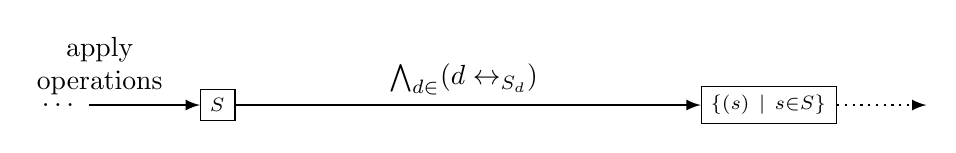
\begin{tikzpicture}[>=latex]
    %\node[draw,align=center] at (3.25, 1.75) {For all $d \in \derivedvars:$\\create BDD $S_d[\vars]$};
    \node[] at (1,0) (dots) {\dots};
    \node[draw] at (3,0) (states) {$\charf_{S}$};
    \node[draw] at (10.0,0) (fullstates) {$\charf_{\{\axioms{}(s) ~\mid~ s \in S\}}$};

    \draw[->, thick] (dots) -- (states) node[pos=0.1,above,align=center] {apply\\operations};
    \draw[->, thick] (states) -- (fullstates) node[midway,above,align=center] {$\bigwedge_{d \in \derivedvars} (d \leftrightarrow \charf_{S_d})$ };
    \draw[->,dotted,thick] (fullstates) -- (12.0,0);
\end{tikzpicture}

    \caption[\vars{}-based encoding of axioms.]{Visualization of symbolic \emph{forward} search with the
        \vars{}-based encoding of axioms \autocite{speck-et-al-icaps2019}.\label{fig:axiom_option2}}
\end{figure}

\medskip
The following two axiom encodings are based on the idea of precomputing a symbolic representation over the primary variables $\vars$ for each derived variable $d \in \derivedvars$ if $d$ is true (\Cref{def:primary_representation}). 
This overcomes the problem of the $\operators$-based encoding, which requires an expensive fixed point computation to be performed in each planning step. 
\textcite{speck-et-al-icaps2019} present an efficient algorithm for computing the primary representation for each derived variable using BDDs.

\begin{definition}[Primary Representation]\label{def:primary_representation}
    Let $d \in \vars \cup \derivedvars$ be a (primary or derived) variable and $\axioms$ a set of axioms.
    The \emph{primary representation} of $d$ is the set of states $S_d$, which contains all states over $\vars$ where $d$ is evaluated to true, i.e., $S_d = \{ s \in \states ~|~ \axioms(s) \models d \}$.
\end{definition}

\paragraph{$\vars$-Based Encoding.}
\Cref{fig:axiom_option2} illustrates the $\vars$-based encoding, where each state of a given set of successor states $S$ is expanded.
Starting from the primary representation (\Cref{def:primary_representation}), the derived variable $d$ in a state $s \in S$ is true if $s \in S_d$. 
Therefore, $\charf_{\{\axioms{}(s) ~\mid~ s \in S\}} = \charf_{S} \land \bigwedge_{d\in \derivedvars} (d \leftrightarrow \charf_{S_d})$ represent the extended set of states. 


\paragraph{Symbolic Translation.}
In contrast to the $\operators$-based and $\vars$-based encodings, the symbolic translation encoding completely omits derived variables by performing the search using a translation of the original planning task.
The idea of the translation is to replace all occurrences of derived variables in the planning task with their corresponding primary representation. In particular, derived variables in operator preconditions and the goal formula are replaced by their corresponding primary representation (\Cref{fig:axiom_option3}). Thus, no reasoning about derived variables during the actual search is required.
%
Note that this symbolic translation encoding is different from compilations that convert \pddl{} with axioms to \pddl{} without axioms \autocite{gazen-knoblock-ecp1997,thiebaux-et-al-aij2005}, since at no point is an explicit version of the compiled task (a new \pddl{} representation) created. 
While the primary representation, and thus the symbolic translation, can lead to exponential size growth in the worst case, in practice it is shown that the concise representation of BDDs alleviates this problem (see Empirical Evaluation).
\medskip

\begin{figure}[t]
    \centering
    \begin{tikzpicture}[>=latex]
	\node[align=center] at (0, 0.65) (tr_before) {
		transition relation\\$\charf_{T_o}$ over $\vars \cup \derivedvars$};
	\node[align=center] at (8, 0.65) (tr_after) {$\charf_{T'_o}$ with complex\\precondition over $\vars$};

	\node[align=center] at (0, -0.75) (goal_before) {goal condition\\$\charf_\goal$ over $\vars \cup \derivedvars$};
	\node[align=center] at (8, -0.75) (goal_after) {complex goal\\ condition $\charf_{\goal'}$ over $\vars$};

	\draw[->, thick] (tr_before) -- (tr_after) node[pos=0.5,above,align=center] {};
	\draw[->, thick] (goal_before) -- (goal_after) node[pos=0.5,above,align=center] {replace all $d \in \derivedvars$\\with $\charf_{S_{d}}$};

	% \node[draw,align=center] at (0, 0.75) (tr_before) {Transition Relation\\$\charf_{T_o}$ over $\vars \cup \derivedvars$};
	% \node[draw,align=center] at (8, 0.75) (tr_after) {$\charf_{T'_o}$ with complex\\precondition over $\vars$};

	% \node[draw,align=center] at (0, -0.75) (goal_before) {Goal condition\\$\charf_\goal$ over $\vars \cup \derivedvars$};
	% \node[draw,align=center] at (8, -0.75) (goal_after) {$\charf_{\goal'}$ with complex\\precondition over $\vars$};

	% \draw[->, thick] (tr_before) -- (tr_after) node[pos=0.5,above,align=center] {};
	% \draw[->, thick] (goal_before) -- (goal_after) node[pos=0.5,above,align=center] {Replace all $d \in \derivedvars$\\with $\charf_{S_{d}}$};
\end{tikzpicture}
    \caption[Symbolic translation encoding of axioms.]{
        Visualization of symbolic \emph{forward}, \emph{backward} and \emph{bidirectional} search with the symbolic translation encoding of axioms \autocite{speck-et-al-icaps2019}.\label{fig:axiom_option3}}
\end{figure}

\textcite{speck-et-al-icaps2019} define the $\operators$-based and the $\vars$-based encoding for symbolic forward search only. It is an open question how to perform backward search, since it is not clear how to efficiently reverse intermediate inferences about the values of derived variables.
In contrast, the symbolic compilation encoding performs all inferences over the derived variables as a preprocessing step. 
Thus, it allows to perform backward search and bidirectional search, which can significantly improve the planning performance.


\paragraph{Empirical Evaluation.}
\Cref{tab:coverage_axioms} shows the coverage (number of optimally solved instances) on different domains with axioms modeling verification problems \autocite{ghosh-et-al-jar2015,edelkamp-icaps2003wscompetition}, multi-agent planning with belief sets \autocite{kominis-geffner-icaps2015} or elevator control \autocite{koehler-schuster-aips2000}. 
Explicit \astar{} search \autocite{hart-et-al-ieeessc1968} is evaluated with the $\heu{blind}{}$ heuristic and the (naive) \heu{max}{} heuristic \autocite{ivankovic-haslum-ijcai2015}, which are the best known heuristics that are admissible and support axioms. 
We see that a BDD-based search is competitive with the $\operators$-based and $\vars$-based approaches compared to the explicit \astar{} search. 
This is mainly due to the good performance in the Miconic Axioms domain, which consists of many instances. 
However, symbolic search using the symbolic translation encoding proves to be the best performing and overall dominant approach, especially with bidirectional search.

%\todo{describe where the domain come from.}

\begin{table}
    \begin{center}
        \resizebox{1\textwidth}{!}{
            \begin{tabular}{lrrccrrr}
    \toprule
    \multirow{2}{*}{Algorithm}               &                                          &                                        & \multicolumn{5}{c}{\textbf{BDD Search}}               \\
    \cmidrule(lr){4-8}

                                            & \multicolumn{2}{c}{\astar{} (explicit)} & \multicolumn{1}{c}{\operators{}-based} &
    {\vars{}-based}                         & \multicolumn{3}{c}{Sym. Translation}                                                                                                      \\

    \cmidrule(lr){2-3} \cmidrule(lr){4-4} \cmidrule(lr){5-5}  \cmidrule(lr){6-8}
    Domain (\#Tasks)                        & \heu{blind}{}                            & \heu{max}{}                            & fwd                                     & fwd & fwd &
    bwd                                     & bid                                                                                                                                       \\
    \midrule
    & \multicolumn{7}{l}{\emph{International Planning Competition (IPC)}} \\
    {Blocks Axioms} (35)             & 18                                       & 18
                                            & 15                                       & 15
                                            & 21                                       & 18                                     &
    \textbf{30}                                                                                                                                                                         \\
    {Grid Axioms} (5)                & 1                                        & 2
                                            & 1                                        & 1
                                            & 1                                        & 0                                      & \textbf{3}                                            \\
    {Miconic Axioms} (150)           & 60                                       & 60
                                            & 127                                      & \textbf{150}
                                            & \textbf{150}                             & \textbf{150}
                                            & \textbf{150}                                                                                                                              \\
    {Optical Telegraphs} (48)        & 2                                        & 2
                                            & 2                                        & 2
                                            & \textbf{4}                               & 0
                                            & \textbf{4}                                                                                                                                \\
    {PSR Middle} (50)                & 35                                       & 35
                                            & 32                                       & 39
                                            & \textbf{50}                              & \textbf{50}
                                            & \textbf{50}                                                                                                                               \\
    {PSR Large} (50)                 & 14                                       & 14
                                            & 13                                       & 15
                                            & 24                                       & 23                                     &
    \textbf{25}                                                                                                                                                                         \\
    {Philosophers} (48)              & 5                                        & 5
                                            & 9                                        & 9
                                            & \textbf{12}                              & 4
                                            & \textbf{12}                                                                                                                               \\
    \midrule
    & \multicolumn{7}{l}{\emph{Complex Preconditions at IPC}} \\
    {Assembly} (30)                  & 0                                        & 0
                                            & 6                                        & 5
                                            & 9                                        & 8                                      &
    \textbf{11}                                                                                                                                                                         \\
    {Airport Adl} (50)               & 19                                       & \textbf{21}
                                            & 14                                       & 12
                                            & 20                                       & 11                                     & 19                                                    \\
    {Trucks} (30)                    & 6                                        & 8
                                            & \textbf{9}                               & \textbf{9}
                                            & \textbf{9}                               & 4
                                            & 8                                                                                                                                         \\
    \midrule
    & \multicolumn{7}{l}{\emph{\textcite{ivankovic-haslum-ijcai2015}}} \\
    {Blocker} (7)                    & \textbf{7}                               &
    \textbf{7}                              & 4                                        & 5
                                            & 5                                        & 5                                      & 5                                                     \\
    {Social Planning} (2)            & \textbf{2}                               &
    \textbf{2}                              & \textbf{2}                               & \textbf{2}
                                            & \textbf{2}                               & \textbf{2}                             & \textbf{2}                                            \\
    {Sokoban Axioms} (25)            & 19                                       & \textbf{20}
                                            & 7                                        & 7
                                            & 18                                       & \textbf{20}
                                            & \textbf{20}                                                                                                                               \\
    \midrule
    & \multicolumn{7}{l}{\emph{\textcite{ghosh-et-al-jar2015}}} \\
    Acc cc2 (7)                    & \textbf{7}                               & \textbf{7}
                                            & \textbf{7}                               &
    \textbf{7}
                                            & \textbf{7}                               & \textbf{7}
                                            & \textbf{7}                                                                                                                                \\
    Grid cc2 (13)                  & \textbf{8}                               & 7
                                            & 0                                        & 0
                                            & 0                                        & 0                                      & 0                                                     \\
    \midrule
    & \multicolumn{7}{l}{\emph{\textcite{kominis-geffner-icaps2015}}} \\
    Collab And Comm (1)            & \textbf{1}                               &
    \textbf{1}                              & 0                                        & 0
                                            & 0                                        & 0                                      & 0                                                     \\
    Muddy Children (1)             & \textbf{1}                               &
    \textbf{1}                              & \textbf{1}                               & \textbf{1}                             & \textbf{1}                              & 0
                                            & \textbf{1}                                                                                                                                \\
    Muddy Child (1)                & \textbf{1}                               &
    \textbf{1}                              & \textbf{1}                               &
    \textbf{1}                              & \textbf{1}                               &
    \textbf{1}                              & \textbf{1}                                                                                                                                \\
    Sum (1)                        & \textbf{1}                               &
    \textbf{1}                              & \textbf{1}                               &
    \textbf{1}                              & \textbf{1}                               & 0
                                            & \textbf{1}                                                                                                                                \\
    Word Rooms (2)                 & \textbf{2}                               &
    \textbf{2}                              & 0                                        & 0
                                            & 0                                        & 0                                      & 0                                                     \\
    \midrule
    w/o Miconic (406) & 149                                      & 154
                                            & 134                                      & 131
                                            & 185                                      & 153                                    &
    \textbf{199}                                                                                                                                                                        \\
    %\midrule
    \textbf{Sum (556)}                      & 209                                      & 214
                                            & 251                                      & 281
                                            & 335                                      & 303                                    &
    \textbf{349}                                                                                                                                                                        \\
    \bottomrule
\end{tabular}

        }
    \end{center}
    \caption[Coverage for planning with axioms.]{Coverage (number of optimally solved instances) for explicit and symbolic search algorithms on domains with axioms \autocite{speck-et-al-icaps2019}.}
    \label{tab:coverage_axioms}
\end{table}

%\section{Summary}